
\chapter{Inleiding}

Routeplanning is momenteel een van de moeilijkste onderzoeksonderwerpen. Dit komt hoofdzakelijk door twee problemen:

\begin{itemize}
\item Een eerste probleem is dat de data moet bestaan. Zo heeft de Belgische spoorwegennetwerk pas in 2015 hun tijdstabellen opgesteld in een uniform formaat.  Om 100\% correcte routeplanning te doen is realtime informatie noodzakelijk. Er zijn maar zeer weinig ov-bedrijven die dit hebben in het juiste formaat en nog minder die dit vrijgegeven.
\item Een twee probleem hierbij is dat deze data geen Open Data is. Sinds augustus 2015 is de Belgische overheid "open-by-default". Dit houdt in dat alle gegevens van de overheid publiek moeten zijn, tenzij explicitiet verklaard wordt waarom deze niet open kan, bijvoorbeeld wegens privacy-schending. Sommige ov-bedrijven zoals De Lijn en de NMBS, geven hun tijdstabellen pas vrij onder 1 op 1 contract waardoor het voor ontwikkelaars moeilijk is om met deze data aan de slag te gaan.\end{itemize}

Deze twee problemen zorgen ervoor dat het zeer moeilijk is om een oplossing te vinden die duurzaam met deze verschillende datasets kan omgaan.

Er komt meer bij routeplanning kijken dan van punt A naar B te geraken via de snelste of kortste weg. We leven in een wereld vol verandering. Nieuwe technologi\"en zoals the Internet Of Things (IOT) zorgen voor nieuwe opportuniteiten. Meer en meer zal data over jou en jouw omgeving een centrale rol spelen. Ook bij routeplanning is personalisatie belangrijk. Dit kan gaan van interessante gebouwen in de buurt tot toegankelijkheid van perrons voor minder valide mensen.

Open Data is sinds kort in een sterke opmars. Zo is er geschat \footnote{http://www.decroo.belgium.be/nl/groen-licht-voor-federale-open-data-strategie-overheidsdata-voortaan-vrij-beschikbaar} dat Belgi\"e een nettowinst van 900 miljoen euro ontloopt door bepaalde datasets niet open te stellen. Er komt een bewustzijn dat het duurzaam oplossen van bepaalde problemen met data moet gebeuren. 

\section{Probleemstelling}
\label{probleemstelling}

Tot voor kort waren er twee mogelijkheden om een routeplanning applicatie te bouwen:
\begin{itemize}
\item ofwel beschikt de cli\"ent over alle data lokaal. Zo kunnen alle behoeften van de cli\"ent voldaan worden. Dit is kostelijk voor de cli\"ent, want alles moet zelf berekend worden. Meestal bevat deze niet over de nodige geheugencapaciteit om routes te berekenen over grote datasets.
\item ofwel wordt er een server opgezet die een bepaalde functionaliteiten aanbiedt, dit onder de vorm van een  Application Programming Interface (API). Zoals je kan zien in \ref{klassieke-webservice-interface} kunnen er meerdere parameters meegegeven worden: waar is het startpunt, wanneer wil je vertrekken, waar wil je aankomen...
\begin{lstlisting}[label=klassieke-webservice-interface,caption=Klassieke webservice interface]
http://my-api.org?start={...}&bestemming={...}&vertrektijd={?}&transportmodes={...}&extraFeature={...}&...
\end{lstlisting}
Er zijn tiental mogelijke modes zoals de bus, boot of trein. Een andere uitdaging van routeplanning is het overstappen tussen twee perrons. Overstappen is voor een bejaarde niet hetzelfde als voor een marathon-loper. Kortom, routeplanning moet met meerdere factoren rekening kunnen houden. Om dit allemaal te berekenen wordt ervoor geopteerd om de server deze berekeningen te laten doen.
Enkele voordelen hiervan:
\begin{itemize}
\item Cli\"ents met weinig rekenkracht kunnen snel routeplanningsadvies bekomen.
\item Er is weinig bandbreedte nodig: 1 HTTP request is voldoende.
\end{itemize}
Er zijn ook enkele nadelen hieraan verbonden:
\begin{itemize}
\item Personalisatie is zeer moeilijk.
\item Een service uitbreiden is moeizaam door de vele factoren die mee rekening gehouden worden.\end{itemize}
\end{itemize}

In figuur \ref{probleemrouteplanning} zie je deze mogelijkheden weergegeven op een Linked Data Fragments-as (LDF). Dit is een conceptueel framework om de balans tussen cli\"ent en server weer te geven. Later (\ref{ldf}) zal dit beter uitgelegd worden.
 \begin{figure}[h!]
\centering
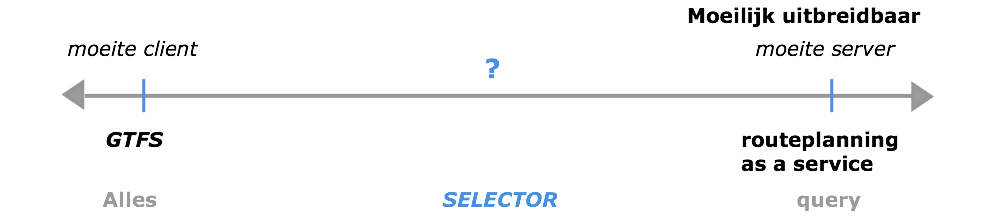
\includegraphics[width=0.8\textwidth]{LDF-as2.png}
\caption{Linked Data Fragments as: huidige oplossingen om routes te plannen. Cli\"ent beschikken ofwel over alle data in een dump, ofwel over een service die het routeplannen voor zich neemt.}
\label{probleemrouteplanning}
\end{figure}

Linked Connections is een manier om transportdata te publiceren zodanig dat het mogelijk is om een route te berekenen hieruit. De basiseenheid is een connectie (zie \ref{connectievb}). Een connectie is de verbinding tussen een vertrek- en eindstop zonder onderbreking, met respectievelijk een vertrek- en aankomsttijd. Een route bestaat uit een combinatie van deze connecties. Connecties zijn gelinkt als ze links bevatten naar andere informatie, zoals connecties die hierop volgen of interessante koffiebars in de buurt.

\begin{figure}[h!]
\centering
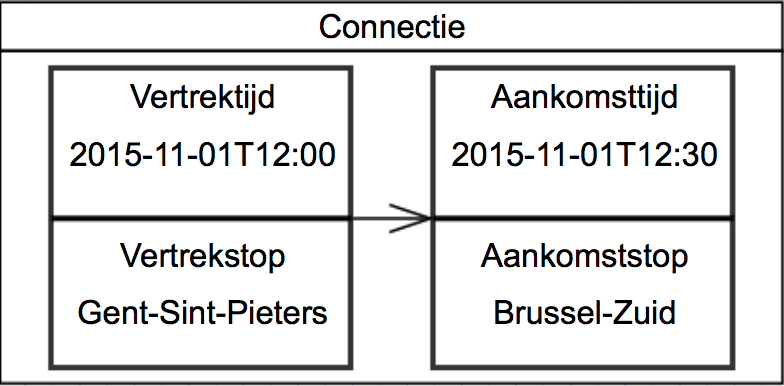
\includegraphics[scale=0.5]{connectie.png}
\caption{Voorbeeld van een connectie. Deze bestaat uit een vertrek- en aankomstplaats, resp. met vertrek- en aankomsttijd}
\label{connectievb}
\end{figure}

Met Linked Connections is het mogelijk om client-side een route te berekenen terwijl server-side connecties ter beschikking stelt. Dit introduceert nieuwe trade-offs die onderzocht kunnen worden. Deze worden weergegeven op de LDF-as \ref{LDF-as3.png}

 \begin{figure}[h!]
\centering
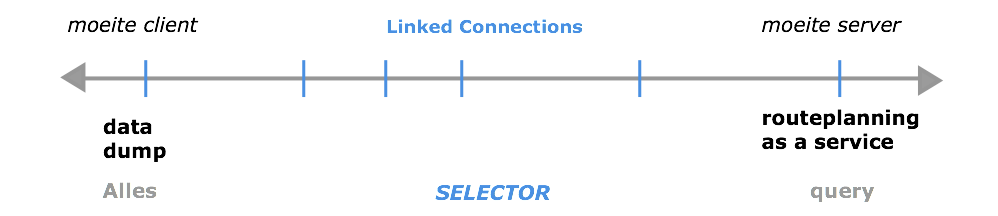
\includegraphics[width=0.8\textwidth]{LDF-as3.png}
\caption{Linked Connections opent nieuwe trade-offs tussen cli\"ent en server aan.}
\label{probleemrouteplanning}
\end{figure}

%\vspace{3mm} %5mm vertical space

De bestaande Linked Connections implementatie werkt momenteel enkel voor een server die connecties ter beschikking stelt. Een probleem hierbij is dat connecties enkel opvraagbaar zijn binnen een tijdsinterval. De cli\"ent wordt overstelpt met connecties die niet nuttig zijn voor het berekenen van de route.

Het doel van deze masterproef is te onderzoeken hoe meerdere datastromen van connecties samengebundeld kunnen worden. Vervolgens wordt onderzocht wat de performantie met de huidige implementatie is en hoe deze verbeterd kan worden.

\section{Onderzoeksvraag}

Deze masterproef zal hoofdzakelijk een antwoord bieden op volgende vraag:
\begin{itemize}
\item \emph{Hoe kunnen we client-side routeplannen met gelinkte connecties sneller maken?}
\end{itemize}

Client-side routeplannen kan sowieso sneller gemaakt worden zoals bij huidige routeplanners het geval is. We willen alle mogelijkheden van het web gebruiken om het publiceren van die gelinkte connecties op de server zo kosteloos mogelijk te maken met daarbij enkele filtermogelijkheden om het routeplannen op de client snel te maken. Verschillende \textit{trade-offs} zullen onderzocht moeten worden.

Enkele subvragen die we hierbij kunnen stellen, zijn:
\begin{enumerate}
\item Welke extra filter(s) moeten toegevoegd worden?
\item Welke metadata kan een meerwaarde bieden voor de cli\"ent?
\item Kunnen we garanderen dat de snelste route gevonden wordt bij extra filtering?
\item Wat is het effect van caching op de berekeningstijd?
\end{enumerate}

\section{Hypotheses}
\label{hypotheses}
Volgende hypotheses zijn waargenomen:
\begin{enumerate}
\item De huidige implementatie met tijdsfilter werkt te traag voor routes over lange afstand.
\item De snelheid van het algoritme hangt af van het aantal connecties die gescand moeten worden. Een request meer sturen is minder erg dan meer connecties per request.
\item Het toevoegen van een extra filter om enkel nuttige connecties op te vragen zal client-side routeplanning minstens dubbel zo snel maken.
\end{enumerate}

Deze hypotheses zullen in hoofdstuk \ref{resultaten} en \ref{hs:conclusie} besproken worden.

\section{Ori\"entatie}

In volgend hoofdstuk komt een uitgebreide literatuurstudie over het semantisch web en technologi\"en die een belangrijke hebben bij routeplanning. In hoofdstuk \ref{lc} worden Linked Connections onder de loep genomen. Hierna wordt een optimalisatietechniek voorgesteld in hoofdstuk \ref{opt}. Als voorlaatste hoofstuk wordt de performantie getest van de oorspronkelijke implementatie en de optimalisatie. Ten slotte, in hoofdstuk \ref{conclusie} wordt een antwoord geformuleerd op de vraag hoe we client-side routeplanner sneller kunnen maken en welke aspecten toekomstig onderzoek vergen.

